% !TeX TXS-program:compile = txs:///xelatex/[--shell-escape]
% IACR Transactions CLASS DOCUMENTATION
% Written by Gaetan Leurent gaetan.leurent@inria.fr (2016-2018)
%
% To the extent possible under law, the author(s) have dedicated all
% copyright and related and neighboring rights to this software to the
% public domain worldwide. This software is distributed without any
% warranty.
%
% You should have received a copy of the CC0 Public Domain Dedication
% along with this software. If not, see
% <http://creativecommons.org/publicdomain/zero/1.0/>.

\documentclass[preprint]{iacrtrans}
\usepackage[utf8]{inputenc}

\setcounter{tocdepth}{4}

%% VERSION
\newcommand{\version}{v.1.0}


%% TITLE
\title{
  
\includegraphics[width=\columnwidth]{logo_zkEVM.png} \\ \vspace{0.3cm}
  Knowledge Layer \\ \vspace{0.3cm}
  Architecture \\ \vspace{0.3cm}
  L2StateTree: Keys and Values \\ \vspace{0.3cm}
  \version
}

\institute{}


\usepackage{caption}
\usepackage{subcaption}

% This package controls how hyperlinks are displayed
% https://es.overleaf.com/learn/latex/Hyperlinks
\usepackage{hyperref}
\hypersetup{colorlinks=true,linkcolor={red!80!black},urlcolor={blue!80!black}}

%Multiple columns
\usepackage{multicol}

% Used for super caligraphic font \mathscr{}
\usepackage{mathrsfs}

%This ensures spaces when using ensuremath and no $$ are used to introduce math
\usepackage{xspace}

%%%%%% BEGIN OF CODE HIGHLIGHTING ENVIRONMENTS %%%%%%

%   sudo apt install texlive-latex-extra
%   sudo apt install python-pip
%   pip install pygments
%   pip install pygments-lexer-babylon  #contains JSX
%   pip install pygments-lexer-solidity
%   pip install pygments pygments-lexer-babylon pygments-lexer-solidity


% *** COLOR COMMANDS ***
\definecolor{dblackcolor}{rgb}{0.0,0.0,0.0}
\definecolor{dbluecolor}{rgb}{0.01,0.02,0.5}
\definecolor{dgreencolor}{rgb}{0.2,0.4,0.0}
\definecolor{dgraycolor}{rgb}{0.30,0.3,0.30}
\newcommand{\dblue}{\color{dbluecolor}\bf}
\newcommand{\dred}{\color{dredcolor}\bf}
\newcommand{\dblack}{\color{dblackcolor}\bf}
\definecolor{light-gray}{gray}{0.96} %the shade of grey that stack exchange uses

\usepackage{showexpl}% already includes listings package
\makeatletter
\def\lst@filenamerpl{_\textunderscore $\textdollar}
\makeatother
\lstset{frame=shadowbox, basicstyle=\footnotesize\ttfamily, showstringspaces=false,
rulesepcolor=\color{black}, upquote=true}

\lstdefinestyle{scriptStyle}{
    basicstyle=\footnotesize,% control font of code
    preset=\footnotesize,% adjust font size of output
    numbers=none,
    frame=tlbr,
    pos=r,% want output on rightbackgroundcolor=\color{yellow!30},
    width=0.50\linewidth,
}

\lstdefinestyle{terms}{
    basicstyle=\scriptsize\ttfamily,% control font of code
    preset=\footnotesize,% adjust font size of output
}

\lstdefinestyle{termt}{
    basicstyle=\footnotesize\ttfamily,% control font of code
    preset=\footnotesize,% adjust font size of output
	numbers=none,
}

\lstdefinestyle{verb}{
    basicstyle=\footnotesize,% control font of code
    preset=\footnotesize,% adjust font size of output
    frame=tlbr,
    pos=r,% want output on right
%     backgroundcolor=\color{yellow!30},
    width=0.50\linewidth,
}

\lstdefinestyle{verbs}{
    basicstyle=\scriptsize,% control font of code
    preset=\scriptsize,% adjust font size of output
    frame=tlbr,
    pos=r,% want output on right
%     backgroundcolor=\color{yellow!30},
    width=0.50\linewidth,
}

\lstdefinestyle{verbt}{
    basicstyle=\tiny\ttfamily,% control font of code
    preset=\tiny\ttfamily,% adjust font size of output
    frame=tlbr,
    pos=r,% want output on right
%     backgroundcolor=\color{yellow!30},
    width=0.50\linewidth,
}

\lstdefinestyle{verbtt}{
    basicstyle=\footnotesize\ttfamily,% control font of code
    preset=\footnotesize\ttfamily,% adjust font size of output
    frame=none,
    pos=r,% want output on right
    xleftmargin=.2\textwidth, xrightmargin=.2\textwidth,
    width=0\linewidth,
}


%Linter for circom
\usepackage{tcolorbox}
\tcbuselibrary{minted,skins,listings}
\definecolor{mybg}{rgb}{0.96,0.96,0.98}
% \lstset{
% 	backgroundcolor = \color{light-gray},
% 	showtabs = False,
% 	tabsize = 2,
% 	showspaces = False,
% 	showstringspaces = False,
% 	commentstyle = {\ttfamily\color{dgreencolor}},
% 	keywordstyle = {\ttfamily\color{dbluecolor}\bfseries},
% 	stringstyle = {\ttfamily\color{dgraycolor}\bfseries},
% 	language = circom,
% 	basicstyle = {\fontsize{7pt}{7pt}\ttfamily},
% 	aboveskip = 1em,
% 	belowskip = 1em,
% 	numbers = left,%none,
% 	numbersep=5pt,    %space line numbers from code
% 	xleftmargin=2em,
% 	frame=single,	% adds a frame around the code
% 	framexleftmargin=1.7em,
% 	numberstyle=\tiny,%\color{gray}
% 	emph = {proc,retp,endp,local},
% 	emphstyle = {\color{blue}\textbf},
% 	literate =
% 		{<==}{{{\color{dbluecolor}<==}}}2
% 		{==>}{{{\color{dbluecolor}==>{}}}}2
% 		{===}{{{\color{dbluecolor}==={}}}}2
% 		{<--}{{{\color{dbluecolor}<---{}}}}2
% 		{-->}{{{\color{dbluecolor}--->{}}}}2
% 		{*}{{{\color{dbluecolor}*{}}}}2
% }

\lstdefinelanguage{circom}{
	keywords=[1]{signal, input, output, public, <==, ==>, ===}, % generic keywords including crypto operations
  	keywordstyle=[1]\color{blue!70!}\bfseries,
	keywords=[3]{pragma, include},
  	keywordstyle=[3]\color{brown}\bfseries,
	keywords=[4]{for, if, var, else},
	keywordstyle=[4]\color{teal}\bfseries,
	keywords=[5]{template, component},
	keywordstyle=[5]\color{violet}\bfseries,
	identifierstyle=\color{black},
	sensitive=false,
	comment=[l]{//},
	morecomment=[s]{/*}{*/},
	commentstyle=\color{green!40!black}\ttfamily,
	stringstyle=\color{blue}\ttfamily,
%	morestring=[b]',
%	morestring=[b]"
}

\newtcblisting{circom}{
  listing engine=listings,
  colback=mybg,
  colframe=black!70,
  listing only,
  listing options={
    language={circom},
	basicstyle=\footnotesize\ttfamily,
    frame=none,
	numbers=none, %left
	numberstyle=\tiny,
	numbersep=9pt,
	tabsize=2,
	breaklines=true,
	showtabs=false,
	captionpos=b
  },
  left=0.2mm,
  top=0cm,
  bottom=0cm,
  boxrule=0.1mm
}

\newtcblisting{js}{
	listing engine=minted,
	colback=mybg,
	colframe=black!30,
	listing only,
	minted style=tango,
	minted language=js,
	minted options={linenos=false,texcl=true},
	left=0.2mm,
	top=0cm,
	bottom=0cm,
	boxrule=0.1mm
}

\lstdefinelanguage{Pil}{
	keywords=[1]{pol, commit, constant, in, is, connect, public, namespace}, % generic keywords including crypto operations
  keywordstyle=[1]\color{blue!70!}\bfseries,
	keywords=[3]{include}, % modules
  keywordstyle=[3]\color{brown}\bfseries,
	keywords=[4]{},% types; money and time units
	keywordstyle=[4]\color{teal}\bfseries,
	keywords=[5]{field, bool, u32, u16, u8},	% environment variables
	keywordstyle=[5]\color{violet}\bfseries,
	identifierstyle=\color{black},
	sensitive=false,
	comment=[l]{//},
	morecomment=[s]{/*}{*/},
	commentstyle=\color{green!40!black}\ttfamily,
	stringstyle=\color{blue}\ttfamily,
%	morestring=[b]',
%	morestring=[b]"
}

\newtcblisting{pil}{
  listing engine=listings,
  colback=mybg,
  colframe=black!70,
  listing only,
  listing options={
    language={Pil},
	basicstyle=\footnotesize\ttfamily,
    frame=none,
	numbers=none,
	numberstyle=\tiny,
	numbersep=9pt,
	tabsize=2,
	breaklines=true,
	showtabs=false,
	captionpos=b
  },
  left=0.2mm,
  top=0cm,
  bottom=0cm,
  boxrule=0.1mm
}

%%%%%%% END OF CODE HIGHLIGHTING ENVIRONMENTS %%%%%%%

\usepackage{url}
\usepackage{tikz}
\usepackage{graphicx} % Required for including images
\usepackage[font=small,labelfont=bf]{caption}  % Required for specifying captions to tables and figures


%%%%%%%%%%%%%%%%%%% BEGIN OF MACROS %%%%%%%%%%%%%%%%%%%

% Cryptocode: https://github.com/arnomi/cryptocode
\usepackage[
lambda,
operators,
landau, %este es el de bigO
probability,
%sets,
logic, %para or,and...
asymptotics,
keys
]{cryptocode}

% My own procedure blocks to show protocols
\createprocedureblock{mypb}{center, boxed}{}{}{linenumbering}
\createprocedureblock{mypbnonum}{center, boxed}{}{}{}

% Numbering style
\renewcommand{\pclnstyle}[1]{\text{#1}}
\renewcommand{\pclnseparator}{.}

% Hyphen inside mathmode
\mathchardef\mhyphen="2D

% Mathbb
\newcommand{\FF}{\ensuremath{\mathbb{F}}\xspace}
\newcommand{\KK}{\ensuremath{\mathbb{K}}\xspace}
\newcommand{\NN}{\ensuremath{\mathbb{N}}\xspace}
\newcommand{\ZZ}{\ensuremath{\mathbb{Z}}\xspace}

% Mathcal
\newcommand{\A}{\ensuremath{\mathcal{A}}\xspace}
\newcommand{\C}{\ensuremath{\mathcal{C}}\xspace}
\newcommand{\E}{\ensuremath{\mathcal{E}}\xspace}
\newcommand{\F}{\ensuremath{\mathcal{F}}\xspace}
\renewcommand{\H}{\ensuremath{\mathcal{H}}\xspace}
\newcommand{\I}{\ensuremath{\mathcal{I}}\xspace}
\renewcommand{\O}{\ensuremath{\mathcal{O}}\xspace}
\renewcommand{\P}{\ensuremath{\mathcal{P}}\xspace}
\newcommand{\R}{\ensuremath{\mathcal{R}}\xspace}
\renewcommand{\S}{\ensuremath{\mathcal{S}}\xspace}
\newcommand{\T}{\ensuremath{\mathcal{T}}\xspace}
\newcommand{\V}{\ensuremath{\mathcal{V}}\xspace}

% Mathscr
% \newcommand{\PPP}{\ensuremath{\mathscr{P}}\xspace}


% Mathfrak
\newcommand{\afr}{\ensuremath{\mathfrak{a}}\xspace}
\newcommand{\bfr}{\ensuremath{\mathfrak{b}}\xspace}

% Caligraphic Combiantions
\DeclareMathAlphabet{\mathpgoth}{OT1}{pgoth}{m}{n}
\newcommand{\plonk}{\ensuremath{\mathcal{P}\mathfrak{lon}\mathcal{K}}\xspace}
\newcommand{\plookup}{\ensuremath{\mathpgoth{plookup}}\xspace}

% Abbreviations
% \newcommand{\Pp}{\ensuremath{\mathcal{P}_{\textsf{poly}}\xspace}}
\newcommand{\MTR}{\ensuremath{\text{MTR}}\xspace}
\newcommand{\MTP}{\ensuremath{\text{MTP}}\xspace}
\newcommand{\LCC}{\ensuremath{\text{LCC}}\xspace}
\newcommand{\FRI}{\ensuremath{\textsf{F}}\xspace}
\newcommand{\z}{\ensuremath{\overline{z}}\xspace}
\newcommand{\fsel}{\ensuremath{f^{\text{sel}}}\xspace}
\newcommand{\tsel}{\ensuremath{t^{\text{sel}}}\xspace}
\newcommand{\Evals}{\ensuremath{\textsf{Evals}}\xspace}
\newcommand{\pparams}{\ensuremath{\text{pp}}\xspace}
\newcommand{\vparams}{\ensuremath{\text{vp}}\xspace}
\newcommand{\pre}{\ensuremath{\text{pre}}\xspace}
\newcommand{\tr}{\ensuremath{\text{tr}}\xspace}
\newcommand{\otr}{\ensuremath{\overline{\text{P}}}\xspace}
\newcommand{\im}{\ensuremath{\text{im}}\xspace}
\newcommand{\seed}{\ensuremath{\textsf{seed}}\xspace}
\newcommand{\transcript}{\ensuremath{\textsf{transcript}}\xspace}
\newcommand{\AIR}{\ensuremath{\textsf{A}}\xspace}
\newcommand{\eAIR}{\ensuremath{\textsf{eA}}\xspace}
\newcommand{\accept}{\ensuremath{\textsf{accept}}\xspace}
\newcommand{\reject}{\ensuremath{\textsf{reject}}\xspace}
\newcommand{\eFRI}{\ensuremath{\epsilon_{\textsf{FRI}}}\xspace}
\newcommand{\eSTARK}{\ensuremath{\epsilon_{\textsf{STARK}}}\xspace}
\newcommand{\eeSTARK}{\ensuremath{\epsilon_{\textsf{eSTARK}}}\xspace}
\newcommand{\eC}{\ensuremath{\epsilon_{\textsf{C}}}\xspace}
\newcommand{\ePlo}{\ensuremath{\epsilon_{\textsf{Plo}}}\xspace}
\newcommand{\eMulEq}{\ensuremath{\epsilon_{\textsf{MulEq}}}\xspace}
\newcommand{\eCon}{\ensuremath{\epsilon_{\textsf{Con}}}\xspace}
\newcommand{\eArgs}{\ensuremath{\epsilon_{\textsf{Args}}}\xspace}
\newcommand{\RS}{\ensuremath{\textsf{RS}[\FF,H,\rho]}\xspace}
\newcommand{\RSK}{\ensuremath{\textsf{RS}[\KK,H,\rho]}\xspace}
\newcommand{\LH}{\ensuremath{\textsf{LH}}\xspace}
\newcommand{\ID}{\ensuremath{\textsf{ID}}\xspace}

% C12
\newcommand{\POSEIDON}{\ensuremath{\texttt{POSEIDON12}}\xspace}
\newcommand{\acode}{\ensuremath{\texttt{a}}\xspace}
\newcommand{\CONST}{\ensuremath{\texttt{C}}\xspace}
\newcommand{\PARTIAL}{\ensuremath{\texttt{PARTIAL}}\xspace}
\newcommand{\CMULADD}{\ensuremath{\texttt{CMULADD}}\xspace}
\newcommand{\EVPOL}{\ensuremath{\texttt{EVPOL4}}\xspace}
\newcommand{\FFT}{\ensuremath{\texttt{FFT4}}\xspace}
\newcommand{\nextStep}{\ensuremath{\textsf{'}}\xspace}
\newcommand{\scale}{\ensuremath{\texttt{s}}\xspace}
\newcommand{\firstW}{\ensuremath{\texttt{firstW}}\xspace}
\newcommand{\firstWSquare}{\ensuremath{\texttt{firstW2}}\xspace}
\newcommand{\incW}{\ensuremath{\texttt{incW}}\xspace}
% Caligraphic Combiantions
 \DeclareMathAlphabet{\mathpgoth}{OT1}{pgoth}{m}{n}

% Abbreviations
\newcommand{\stoc}{\texttt{S2C}\xspace}
\newcommand{\ctos}{\texttt{C2S}\xspace}


% Make a nice emptyset
\let\oldemptyset\emptyset
\let\emptyset\varnothing

% Make a nice phi and epsilon
\let\oldphi\phi
\let\phi\varphi
\let\oldepsilon\epsilon
\let\epsilon\varepsilon

% Make a nice q.e.d. symbol
\renewcommand\qedsymbol{\ensuremath{\blacksquare}\xspace}

\theoremstyle{definition}
\newtheorem{protocol}{Protocol}
\newtheorem{bremark}{Remark}

\usepackage{paralist} % for compactitem environment

%%%%%%%%%%%%%%%%%%% END OF MACROS %%%%%%%%%%%%%%%%%%%

% \begin{pcvstack}[boxed, center]
% % \pcsetargs{codesize=\scriptsize{}}

% \procedure{}{
%   \textbf{Prover } \P(g_1(x))  \< \< \textbf{verifier } \V(g_1(x)) \\[][\hline]
%   \< \sendmessageright{top={$f_1(s)$, $f_2(s)$}} \< \\[-2mm]
%   \< \sendmessageleft{top={randomness}} \< \\[-2mm]
%   \< \sendmessageright{top={$f_3(s)$}} \< \\[-2mm]
%   \< \< \text{Samples a random } z \in \FF \text{ and computes } z\vec{g}. \\[-2mm]
%   \< \sendmessageleft{top={$z$}} \< \\[-2mm]
%   \text{Computes evaluations:} \< \< \\
%   \t g_1(z), f_1(z), f_2(z), f_3(z) \< \< \\[-2mm]
%   \< \sendmessageright{top={$g_1(z)$, $f_1(z)$, $f_2(z)$, $f_3(z)$}} \< \\[-2mm]
%   \< \sendmessageleft{top={$v$}} \< \\[-2mm]
%   \< \sendmessageright{top={$\pi$}} \< \\[-2mm]
%   \< \< \text{Verifies the opening proof } \pi \text{ and checks that:} \\
%   \< \< \t g_1(z)(f_1(z) + f_2(z)) - f_3(z) = 0
% }
% \end{pcvstack}

\newcommand{\definedir}[2]{\newcommand{#1}{#2}}
\definedir{\topicdir}{..}
\definedir{\zkevmdir}{../../../..}



\begin{document}
\begin{titlepage}
\centering
\maketitle
\today
\end{titlepage}

% use optional argument because the \LaTeX command breaks the PDF keywords
% \keywords[\publname, ToSC, TCHES, LaTeX]{TBD \and TBD}

%{\hypersetup{linkcolor=.}\tableofcontents}

\newpage
% !TeX spellcheck = en_GB
% !TeX TXS-program:compile = txs:///xelatex/[--shell-escape]
% !TeX root = ../build/l2-state-storage.tex




%%%%%%%%%%%%%%%%%%%%%%%%%%%%%%%%%%%%%%%%%%%%%%%%%%%%%%%%%%%%%%%%%%%%%%%%%%%
\section{A zk-Friendly Sparse Merkle Trie for the zkEVM State}

The Merkle tree we are using to store the zkEVM State is a Sparse Merkle Binary Trie fully updatable (that is, allowing both read and write operations)  used to represent key-value data. We will also make it radix in order to optimize storage space. Due to its construction, it will be unbalanced by nature (since keys, which are used to completely locate leaves within the tree, will be hashes of some data).

\paragraph*{Underlying Hash Function}

\texttt{Poseidon} is a cryptographic hash function that has garnered attention for its unique properties and suitability in the context of Zero-Knowledge proofs. It was originally designed to address some of the limitations and challenges faced by traditional hash functions in this specific application domain. From now on, we will consider an instantiation of \texttt{Poseidon} over a Goldilocks field (that is, $\FF_p$ where $p = 2^{64} - 2^{32} + 1$), that takes as entry $8$ field elements divided into two groups: four of them are know as \textbf{capacity elements}, and the other $4$ are the elements to be hashed, known as \textbf{input elements} and outputs $4$ field elements known as \textbf{output elements}. We will denote a Poseidon hash as follows:

\[
\texttt{Poseidon}(\texttt{capacity};\texttt{values})
\]

Here, $\texttt{capacity}$ is an array of $4$ field elements representing the capacity elements, and $\texttt{values}$ is an array of $4$ field elements representing the inputs of the hash. Observe that we can also see \texttt{values} as an array of $8$ (almost) $32$-bits elements. In our context, two instances of Poseidon hash function are employed for protecting the tree against second-preimage attacks: $\texttt{Poseidon}(0; \cdot)$ for branch nodes and $\texttt{Poseidon}(1; \cdot)$ for leaf nodes.


\paragraph*{A Glimpse Through Toy Example}

Let's visualize the tree using an example. Lets suppose we have some set of data associated with four keys: \texttt{000110}, \texttt{001011}, \texttt{001100}, and \texttt{101101}. Prefixes are used to position the leaves containing data. We have four distinct prefixes: \texttt{000}, \texttt{0010}, \texttt{0011}, and \texttt{1}. Recall that zero nodes are used to signify the absence of keys under a given prefix. With this design, similar keys share a common path in the tree, saving space.

\begin{figure}[H]
\centering
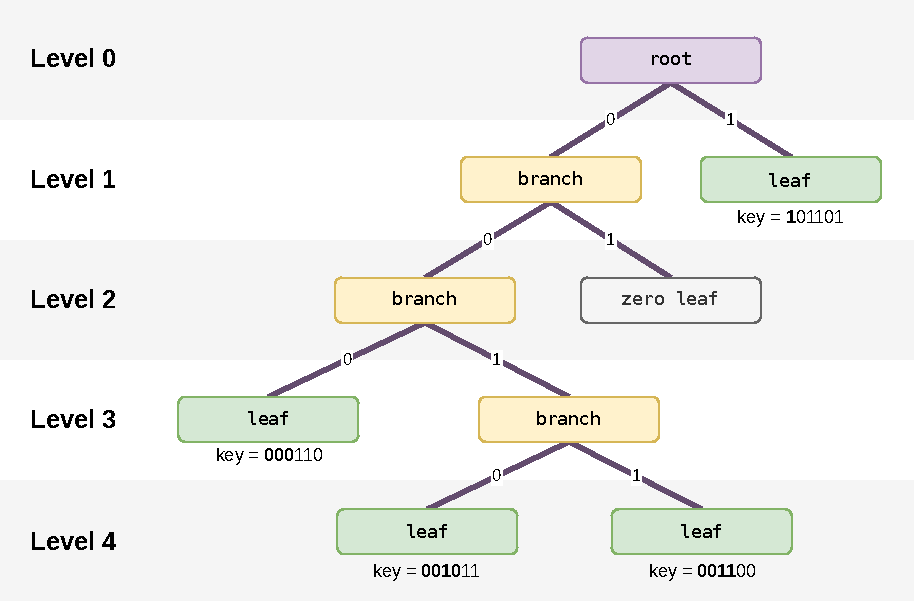
\includegraphics[width=.8\columnwidth]{\zkevmdir/figures/architecture/trie-smt/smt-trie.drawio}
\caption{Illustrative Example of a Sparse Merkle Trie.}
\end{figure}

\paragraph*{The Four Node Types} In the proposed example we can see the $4$ different types of nodes appearing in our tree design:

\begin{itemize}

\item \textbf{Root node}: The root node is the top node of the tree, the only one node at level zero, connecting all branches and leaves. It is the starting point for traversing the tree structure. It serves as a cryptographic summary of all the tree, the final hash of the entire dataset.

\item \textbf{Leaf node}: Leaf nodes encapsulate the actual data associated with a key. Its stored value can be obtained by hashing unique information of each key-value binding of the dataset.

\item \textbf{Branch node}: Branch nodes serve as intermediaries within the tree structure, positioned at various levels between the root node and the leaf nodes. These nodes actively guide the traversal path within the trie. The primary responsibility of a branch node is to store the hash derived from concatenating the hashes of its two child nodes. This hash encapsulates the segment of the cryptographic summary representing the data contained in the subtree rooted at that branch node.

\item \textbf{Zero node}: Zero nodes \textbf{do not} represents a zero value for a specific key. Instead, they denote the absence of a subtree beneath a branch node. In our example, we can see that all keys starting with $01$ share the default value of $0$. Consequently, there is no need for these keys to be individually present as nodes in the tree, and this is where zero nodes come into play. However, the tree actually stores several keys starting with $00$. These keys require the presence of a branch node at level $2$ to obtain the parent's node hash. The optimization lies in the decision not to hash the subtree below with hashes of zero but rather to represent it with an explicit zero value. In practical terms, this means that the branch node at level $1$ assumes a specific value:
\[
\texttt{Poseidon}(0; \texttt{leftChildNode}, 0).
\]

This optimization is called \textbf{partial tree construction}.

\end{itemize}


% !TeX spellcheck = en_GB
% !TeX TXS-program:compile = txs:///xelatex/[--shell-escape]
% !TeX root = ../build/l2-state-storage.tex




\section{Keys and Values}

In the context of managing key-value data within a Merkle tree structure, it is important to correctly specify the process by which keys and values are employed to create and position data within the tree. The leaf nodes serve as the endpoints of the tree and essentially hold data.

\subsection{Obtaining the Keys}

The current methodology employed for hashing the leaf data to derive the node's key unfolds as follows:

$$ \texttt{leafKey} = \texttt{Poseidon}(\texttt{capacityHash}; \texttt{addr}, \texttt{SMT\_KEY}, 0) $$

The array

$$ \texttt{addr} = (\texttt{addr[0]}, \texttt{addr[1]}, \texttt{addr[2]}, \texttt{addr[3]}, \texttt{addr[4]}) $$

comprises a 32-bit segmented representation of the Ethereum address associated with the leaf, having $160$ bits in the EVM. $\texttt{SMT\_KEY}$ is a single field element that takes the following values for the different L2
state information being stored:

\begin{itemize}
\item \texttt{SMT\_KEY = 0}: for the account balances.
\item \texttt{SMT\_KEY = 1}: for the account nonces.
\item \texttt{SMT\_KEY = 2}: for the smart contracts' code.
\item \texttt{SMT\_KEY = 3}: for the smart contracts' storage.
\item \texttt{SMT\_KEY = 4}: for the smart contracts' length.
\end{itemize}

The computation of the capacity hash differs depending on whether we are storing a storage slot or some other type of data.

\begin{enumerate}[(a)]

\item When storing data that is not a storage slot, the capacity hash is computed as follows:
\[
\texttt{capacityHash}  = \texttt{Poseidon}(0; 0),
\]
where the capacity shown as \texttt{0} is an array of $4$ field elements all of them set to $0$.

\item Since a single smart contract's address can have multiple storage slots, we create different keys for each slot as follows:
\[
\texttt{capacityHash} = \texttt{Poseidon}(0; \texttt{storageKey}),
\]
where \texttt{storageKey} is an array of $8$ field elements where each of these elements is constrained to values of $32$ bits for the representation of the storage slot identifiers, which in the EVM have a size of $256$-bits.

\end{enumerate}


\subsection{Obtaining the Values}

Having specified the procedure for deriving the keys associated with the leaves, it is equally important to outline the process by which the values stored within these leaves are obtained. The current methodology employed for hashing the leaf data to derive the node's value unfolds as follows:
\[
\texttt{leafValue} = \texttt{Poseidon}(1; \texttt{remLeafKey}, \texttt{valueHash}).
\]

In this case, the capacity $\texttt{1}$ is an array of 4 field elements with $\texttt{c}[0] = 1$ and $\texttt{c}[1] = \texttt{c}[2] = \texttt{c}[3] = 0$. The \texttt{remLeafKey} argument of the hash consists as an array of $4$ field elements, which collectively represent the remaining key associated with the leaf node. The second argument \texttt{valueHash} is is an array of 4 field elements that is calculated as follows:
\[
\texttt{valueHash} = \texttt{Poseidon}(0; \texttt{value}),
\]
where $\texttt{value}$ is an array of 8 field elements, with each element constrained to values of 32 bits. The $32$-bits values in the array are computed differently depending on the type of the data intended for storage within the tree.:

\begin{itemize}

\item \textbf{\texttt{balances}, \texttt{nonces} and \texttt{storageSlotValues}.}

In the EVM, \texttt{balances}, \texttt{nonces} and \texttt{storageSlotValues} are of $256$ bits. So, their \texttt{valueHashes} are computed as expected:
\begin{align*}
\texttt{valueHash} &= \texttt{Poseidon(0; balance)}, \\
\texttt{valueHash} &= \texttt{Poseidon(0; nonce)}, \\
\texttt{valueHash} &= \texttt{Poseidon(0; storageSlotValue)}.
\end{align*}

All the previous arrays are of 8 field elements constrained to values of 32 bits.

\item \textbf{Smart Contracts Code.}

In the L2 state tree we also need to store the hash of the smart contracts’ bytecode. The issue is that the bytecode of smart contract can be larger than $256$-bits ($32$ bytes). Actually, it can have an arbitrary size. To manage these issues:

\begin{itemize}

\item We use a \textbf{padding} to complete the size of data being hashed to a multiple of a suitable size that is $56$ bytes (we see why next).

\item Then, we linearly hash the resulting padded byte string.

\end{itemize}

\begin{figure}[H]
\centering
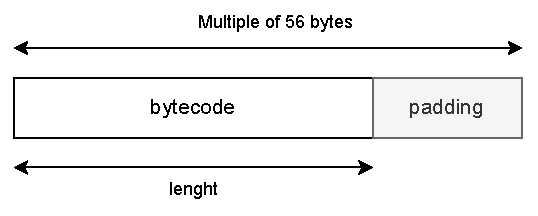
\includegraphics[width=0.5\columnwidth]{\zkevmdir/figures/architecture/L2StateTree/bytecode-padding.drawio}
\caption{The padding is introduced in order to enable the bytecode to be hashed using \texttt{Poseidon}. }
\label{fig:padding}
\end{figure}
In the L2 state tree, we also need to store the bytecode length to distinguish what is payload from what is padding:

\begin{itemize}

\item The bytecode length represents the number of bytes of the bytecode.

\item This is a 256-bit value.

\item The \texttt{valueHash} is computed as follows:
\[
\texttt{valueHash} = \texttt{Poseidon(0;} \texttt{bytecodeLength}).
\]

\end{itemize}

We encode the bytecode (which is multiple of a byte) in segments of 7 bytes (56 bits), which is the biggest amount of bytes that can be represented with an element of our field:
\[
2^{56} < 2^{64} - 2^{32} + 1 < 2^{64}.
\]

The \texttt{Poseidon} hash function signature that use has 8 inputs, so we hash in blocks of 8 field elements which encode $7\,$ bytes $\times\, 8\,$ elements $= 56$ bytes of bytecode. So, we use a padding procedure that completes the original bytecode string to a padded string that is multiple of 56 bytes as follows:

\begin{enumerate}
\item Add the byte \texttt{0x01} at the end of the original bytecode.
\item Fill with zeros until the padded bytecode length + 1 is multiple of 56 bytes.
\item Add \texttt{0x80} as the last byte.
\end{enumerate}

For example, if the original bytecode is \texttt{0xdead}, having size of $2$ bytes, the padded bytecode becomes \texttt{0xdead01000000000000000000...000000000000080}, having size of $56$ bytes.

Since smart contract's bytecode can be larger than $256$ bits, we will need a chained hash process in order to obtain a valid representative value (that we will call \texttt{bytecodeHash}). More specifically, we recursively hash $8$ of the $7$ bytes segments along with the hash of the preceding chunk, input as the capacity element.

\begin{figure}[H]
\centering
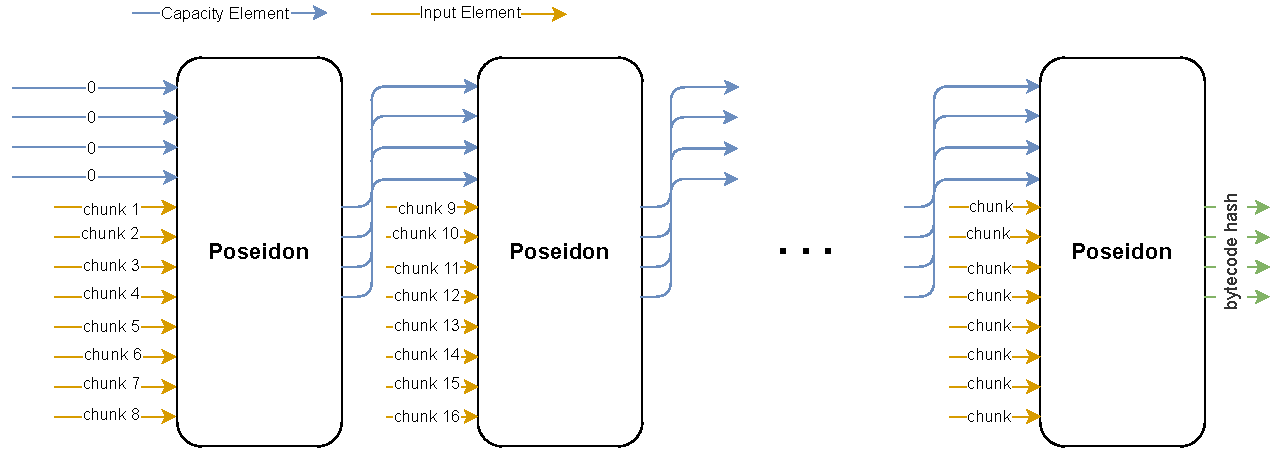
\includegraphics[width=.9\columnwidth]{\zkevmdir/figures/architecture/L2StateTree/bytecode-linear-hash.drawio}
\caption{Notice that we use the output of the previous \texttt{Poseidon} function as the capacity in the new computation of the next \texttt{Poseidon} hash.}
\label{fig:linear-hash}
\end{figure}

Following the previous example having \texttt{0xdead} as the bytecode. Recall that the padded bytecode became
\[
\texttt{0xdead010000000000000000000000000...000000000000000000000080}.
\]
We perform one \texttt{Poseidon} (since the padded bytecode has length $56$ bytes) with the following $12$ elements:

\begin{figure}[H]
\centering
\begin{lstlisting}[style=verbtt]
[ "00000000000000", (7 bytes) (element 0)
  "00000000000000", (7 bytes) (element 1)
  "00000000000000", (7 bytes) (element 2)
  "00000000000000", (7 bytes) (element 3)
  "0000000001adde"  (7 bytes) (element 4)
  "00000000000000"  (7 bytes) (element 5)
  "00000000000000"  (7 bytes) (element 6)
  "00000000000000"  (7 bytes) (element 7)
  "00000000000000"  (7 bytes) (element 8)
  "00000000000000"  (7 bytes) (element 9)
  "00000000000000"  (7 bytes) (element 10)
  "80000000000000"  (7 bytes) (element 11) ]
\end{lstlisting}
\caption{The \texttt{Poseidon} hash is performed with 12 elements, each representing a 7-byte value. Since we are performing the first $7$ bytes, we leave the capacity to $\texttt{0}$. }
\label{fig:example}
\end{figure}

Finally, the \texttt{valueHash} of the bytecode is  \texttt{valueHash} = \texttt{Poseidon(0;} \texttt{bytecodeHash}).

\end{itemize}

\end{document}